\section*{CHAPTER 1: THEORETICAL BACKGROUND}
\addcontentsline{toc}{section}{\numberline{}CHAPTER 1:THEORETICAL BACKGROUND}
\setcounter{section}{1}
\setcounter{subsection}{0}
\setcounter{figure}{0}
\setcounter{table}{0}

This chapter focuses on providing the theoretical foundations and background knowledge necessary to understand the concepts and methodologies discussed in the subsequent chapters of this project.

\subsection{Single-carrier modulation}
% In digital communications, information is expressed in the form of bits. The term symbol refers to a collection, in various sizes, of bits \cite{Litwin2001}.
% In Single-carrier modulation, only one Radio Frequency (RF) carrier is used to carry the information.
In Single-carrier modulation, the signal is transmitted across the entire bandwidth $B$ \cite{OFDM2006}, meaning that only one carrier frequency is used to carry the information. The system's sampling frequency is equal to the bandwidth, and each symbol has a duration of:
\begin{equation}
    T_{SC} = \frac{1}{B}
    \label{eq:single-carrier}
\end{equation}

In Equation \ref{eq:single-carrier}, $T_{SC}$ is the symbol duration, measured in seconds (s); $B$ is the total bandwidth of the system, measured in Hertz (Hz). The power spectral density of single-carrier transmission system is described in Figure \ref{fig:single-carrier}, in which the entire system is modulated with the carrier signal $f_0$. In broadband wireless communication, the radio channel is usually frequency selective, meaning that the channel impulse response varies with frequency. The sampling frequency is very high, resulting in the sample duration $T_{SC}$ being very small, therefore single-carrier modulation technique has several disadvantages:

\begin{itemize}
    \item Inter-symbol interference (ISI), caused by multipath fading. This is because the ratio of the maximal time delay of the channel $\tau_{max}$ to the symbol duration $T_{SC}$:
    \begin{equation}
        R_{SC} = \frac{\tau_{max}}{T_{SC}} = R_{ISI}
    \end{equation}
    This ratio is much larger compared to multi-carrier modulation. The symbol period $T_{SC}$ must be much greater than maximal time delay $\tau_{max}$ in order to avoid ISI at the receiver.
    \item Low data rate: since data rate is inversely proportional to symbol period, having long symbol periods means low data rate and communication inefficiency.
\end{itemize}

Nowadays, single-carrier modulation technique is being use in satellite, GSM, CDMA, HF and other narrowband communication systems \cite{rfwireless}. In broadband communications, multi-carrier system, such as FDM is developed to address the disadvantages discussed above.

\begin{figure}[htbp]
    \centering
    \includegraphics[width=\linewidth]{Figures/single_carrier}
    \caption{Power spectral density of single-carrier transmission system}
    \label{fig:single-carrier}
\end{figure}

\subsection{Multi-carrier modulation}
Frequency division multiplexing (FDM) is a multi-carrier modulation technique by which the total bandwidth $B$ of the system is divided into a series of non-overlapping sub-carrier frequencies, each of which is used to carry a separate signal \cite{b2}. The overall concept of an multi-carrier transmission system is described in Figure \ref{fig:FDM}.

\begin{figure}[htbp]
    \centering
    \includegraphics[width=\linewidth]{Figures/FDM}
    \caption{Power spectral density of multi-carrier transmission system}
    \label{fig:FDM}
\end{figure}

In Figure \ref{fig:FDM}, the data stream is transmitted on $N_C = 2L + 1$ parallel channels with a smaller bandwidth $f_s$:
\begin{equation}
    f_s = \frac{B}{N_C}
\end{equation}

The symbol duration is larger than before:

\begin{equation}
    T_{MC} = T_{SC} N_C
\end{equation}

This results in the ratio of the maximal time delay of the channel $\tau_{max}$ to the symbol duration $T_{MC}$ being much smaller compared to single-carrier modulation:

\begin{equation}
    R_{MC} = \frac{\tau_{max}}{T_{MC}} = \frac{R{SC}}{N_C}
\end{equation}

Thereby the affect of ISI is significantly reduced. Some addition advantages of Frequency Division Multiplexing including:
\begin{itemize}
    \item Allows multiple signals to be transmitted over a single communication channel, which can lead to more efficient use of available bandwidth.
    \item The Frequency selectivity effect is reduced, meaning the channel impulse response affects just a few symbols.
    \item Low Implementation Cost: FDM is a relatively simple technique that does not require sophisticated hardware or software, making it less expensive to implement.
\end{itemize}
However, Frequency Division Multiplexing still has some drawbacks, such as: 
\begin{itemize}
    \item More sensitive to the time variations of the channel (Time selectivity effect).
    \item Interference: FDM can be susceptible to interference from other signals transmitted on nearby frequencies, which can degrade the quality of the transmitted signals.
\end{itemize}

An overall high data rate can be achieved by placing carriers closely in the spectrum. However, inter-carrier interference (ICI) will occur due to a lack of spacing to separate the carriers \cite{ICI}. To avoid inter-carrier interference, guard bands will need to be placed in between any adjacent carriers, which results in a lowered data rate. To address this issue, the Orthogonal Frequency Division Multiplexing (OFDM) method was introduced.

\subsection{Orthogonal Frequency Division Multiplexing modulation}
Orthogonal Frequency Division Multiplexing (OFDM) is a special case of the Frequency Division Multiplexing (FDM) technique \cite{OFDM2010}, with one crucial difference: the subcarriers in frequency domain are overlapping. More specifically, the subcarriers are orthogonal to each other, as described in Figure \ref{fig:OFDM}.

\begin{figure}[htbp]
    \centering
    \includegraphics[width=\linewidth]{Figures/OFDM}
    \caption{Power spectral density of OFDM signal}
    \label{fig:OFDM}
\end{figure}

Figure \ref{fig:sinx} illustrated the principle of the orthogonality, in which the spectrum of a single subcarrier signal has the form of a $sinc(x)$ function, defined in Equation \ref{eq:sinc}. The subcarriers are distributed evenly across the frequency range, ensuring that the peak points of one channel coincide with the null points of adjacent subcarrier channels. In the OFDM system, the signals, after passing through the digital modulator, undergo an Inverse Fast Fourier Transform (IFFT) to form OFDM symbols. The use of IFFT allows the OFDM modulator to simultaneously modulate multiple channels, a task that is challenging with FDM modulators.
\begin{align}\label{eq:sinc}
    sinc(x) =
    \begin{cases}
        \frac{sin(x)}{x} &\text{if} \quad x \neq 0\\
        1 &\text{if} \quad x = 0
    \end{cases}
\end{align}

The key to OFDM is maintaining the orthogonality of the subcarriers. This is important because it prevents subcarriers from disturbing each other and inter-carrier guard bands are not required \cite{wikiOFDM}. If the integral of the product of two signals is zero over a time period, then these two signals are said to be orthogonal to each other. Two sinusoids with frequencies that are integer multiples of a common frequency can satisfy this criterion. The orthogonality is defined in Equation \ref{eq:orthogonality}

\begin{equation}\label{eq:orthogonality}
    \int_{0}^{T} cos(2 \pi n f_o t) cos(2 \pi m f_o t) \,dt = 0 \quad (n \neq m)
\end{equation}

Where $n$ and $m$ are two unequal integers; $f_o$ is the fundamental frequency; $T$ is the period over which the integration is taken. For OFDM, $T$ is one symbol period and $f_o$ set to to $\nicefrac{1}{T}$ for optimal effectiveness.

\begin{figure}[htbp]
    \centering
    \begin{subfigure}[t]{.49\linewidth}
        \includegraphics[width=\linewidth]{../Source/results/sinc1}
        \caption{Spectrum of a single subcarrier}
        \label{fig:single}
    \end{subfigure}
    \hfil
    \begin{subfigure}[t]{0.49\linewidth}
        \includegraphics[width=\linewidth]{../Source/results/sinc2}
        \caption{Spectrum of a four subcarriers}
        \label{fig:four}
    \end{subfigure}
    \caption{Spectrum of a single subcarrier and four subcarriers}
    \label{fig:sinx}
\end{figure}

% Upgrading and optimizing algorithms,
OFDM systems provide highly advantageous features for wireless transmission and transceiver system design:

\begin{itemize}
    \item Since the symbol duration is inversely proportional to the symbol rate, each subcarrier has relatively long symbols. Long symbols are robust against multipath fading, as it occurs in wireless systems.
    \item When a carrier is in a deep fade due to frequency-selectivity of the channel (i.e. the received energy on this carrier is very low), only the data on this subcarrier is lost, instead of the whole stream.
    \item Multicarrier systems allow easy multi-user resource sharing by allocating different subcarriers to different users.
\end{itemize}
However, OFDM technology also has its drawbacks that need careful consideration and practical research for designing a system suitable for specific purposes:
\begin{itemize}
    \item Uneven Amplitude Envelope: The amplitude envelope of the signal is uneven, causing nonlinear distortion in power amplifiers at the transmitter and receiver.
    \item Guard Interval Impact on Transmission Efficiency: While the guard interval is used to eliminate ISI, it also reduces transmission efficiency due to wasting power on transmitting useless signals.
    \item Orthogonality Conditions between Subcarriers: The requirement for orthogonality between subcarriers makes the system susceptible to the effects of Doppler, frequency offset, and time offset due to synchronization errors.
\end{itemize}
These challenges require careful consideration and research to optimize the performance of the OFDM system under real-world conditions and ensure that the drawbacks do not significantly affect transmission quality


\subsection{Cyclic prefix}
OFDM data are generated by taking symbols in the spectral space using M-PSK, QAM, etc, and convert the spectra to time domain by taking the Inverse Discrete Fourier Transform (IDFT). Since Inverse Fast Fourier Transform (IFFT) is more cost effective to implement, it is usually used instead \cite{b3}. Once the OFDM data are modulated to time signal, all carriers transmit in parallel to fully occupy the available frequency bandwidth. During modulation, OFDM symbols are typically divided into frames, so that the data will be modulated frame by frame in order for the received signal be in sync with the receiver. Long symbol periods diminish the probability of having inter-symbol interference, but could not eliminate it. To make ISI nearly eliminated, a cyclic prefix (CP) is added to each symbol period. An exact copy of a fraction of the cycle, typically 25\% of the cycle, taken from the end is added to the front. This allows the demodulator to capture the symbol period with an uncertainty of up to the length of a cyclic extension and still obtain the correct information for the entire symbol period.

\begin{figure}[ht]
    \centering
    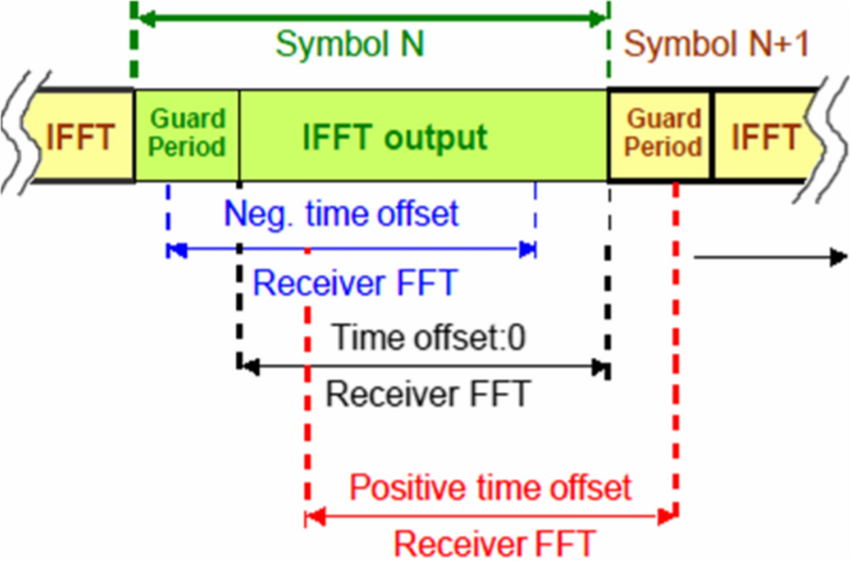
\includegraphics[width=0.5\textwidth]{Figures/Cyclic-extension-tolerance}
    \caption{Cyclic prefix tolerance}
    \label{Cyclic-extension-tolerance}
\end{figure}

As shown in Figure \ref{Cyclic-extension-tolerance}, a guard period, another name for the cyclic extension, is the amount of uncertainty allowed for the receiver to capture the starting point of a symbol period, such that the result of FFT still has the correct information. In Figure 2, a comparison between a precisely detected symbol period and a delayed detection illustrates the effectiveness of the cyclic extension.

\begin{figure}[ht]
    \centering
    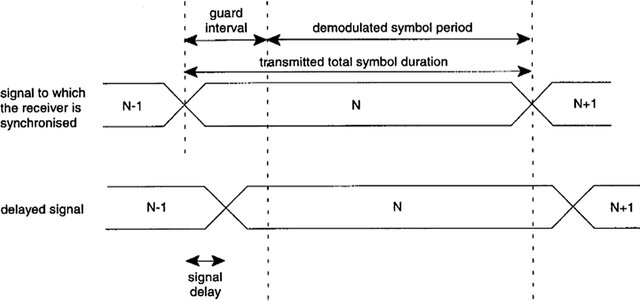
\includegraphics[width=\textwidth]{Figures/Effectiveness-of-cyclic-extension}
    \caption{Effectiveness-of-cyclic-extension}
    \label{Effectiveness-of-cyclic-extension}
\end{figure}
% \subsubsection{Complexity}

% The number of carriers in an OFDM system is not only limited by the available spectral bandwidth, but also by the IFFT size, which is determined by the complexity of the system. The more complex (also more costly) the OFDM system is, the higher IFFT size it has; thus a higher number of carriers can be used, and higher data transmission rate achieved.
% % The choice of M-PSK modulation varies the data rate and Bit Error Rate (BER). The higher order of PSK leads to larger symbol size, thus less number of symbols needed to be transmitted, and higher data rate is achieved. But this results in a higher BER since the range of 0-360 degrees of phases will be divided into more sub-regions, and the smaller size of sub-regions is required, thereby received phases have higher chances to be decoded incorrectly.
% OFDM signals have high peak-to-average ratio, therefore it has a relatively high tolerance of peak power clipping due to transmission limitations.

% \subsection{Conclusion}

% In conclusion, chapter 1 has provided a comprehensive theoretical background necessary for understanding the concepts and methodologies explored in this project, such as: FDM, OFDM, FFT. Now we move on to the next chapter, where we're going to survey some of the existing paper recognition methods and our own proposed methods.

\newpage
